\chapter{Implementacija i korisničko sučelje}
		
		
		\section{Korištene tehnologije i alati}
		
			
			\noindent Komunikacija u timu je ostvarena putem aplikacija \underline{WhatsApp}\footnote{https://www.whatsapp.com/} i \underline{Microsoft Teams}\footnote{https://www.microsoft.com/hr-hr/microsoft-365/microsoft-teams/group-chat-software}. Aplikacija WhatsApp korištena je isključivo za slikovno-tekstualnu komunikaciju, dok je Microsoft Teams korišten za telekonferencijski kontakt. Kao sustav za upravljanje izvornim kodom korišten je \underline{Git}\footnote{https://git-scm.com/}, dok se udaljeni repozitorij projekta nalazi na web platformi \underline{Git Lab}\footnote{https://about.gitlab.com/}. Za izradu UML dijagrama korišten je \underline{Astah UML}\footnote{https://astah.net/}.
			
			\noindent Od alata za razvojno okruženje korišteni su \underline{PyCharm}\footnote{https://www.jetbrains.com/pycharm/} i \underline{Notepad++}\footnote{https://notepad-plus-plus.org/downloads/}. PyCharm je razvojno sučelje koje se koristi za programiranje u Pythonu. Od velike je pomoći kod pisanja koda s laganom navigacijom unutar programa. Notepad++ je dobar za uređenje teksta i izvornog koda za upotrebu u sustavu Microsoft Windows.
			
			\noindent Korištena baza podataka je \underline{PostgreSQL}\footnote{https://www.postgresql.org/}, a nalazi se na poslužitelju u oblaku \underline{Heroku}\footnote{https://www.heroku.com/}.
			
			\noindent Za izradu backenda korišteni su \underline{Python}\footnote{https://www.python.org/} i \underline{Django}\footnote{https://www.djangoproject.com/}, a za frontend \underline{Bootstrap}\footnote{https://getbootstrap.com/}.
			
			\noindent Python (Guido van Rossum, 1990.) programski je jezik opće namjene koji dopušta nekoliko stilova programiranja (objektno orijentirano, strukturno i aspektno orijentirano programiranje).
			
			\noindent Django je besplatan i open-source web framework koji se temelji na Pythonu. Olakšava stvaranje složenih web stanica.
			
			\noindent Bootstrap je frontend framework i besplatna open-source kolekcija HTML CSS i java script alata za kreiranje web stranica i web aplikacija.
			
			\noindent Za pisanje dokumentacije korišten je alat TeXstudio.
			
			
			
			\eject 
		
	
		\section{Ispitivanje programskog rješenja}
			
			\textbf{\textit{dio 2. revizije}}\\
			
			 \textit{U ovom poglavlju je potrebno opisati provedbu ispitivanja implementiranih funkcionalnosti na razini komponenti i na razini cijelog sustava s prikazom odabranih ispitnih slučajeva. Studenti trebaju ispitati temeljnu funkcionalnost i rubne uvjete.}
	
			
			\subsection{Ispitivanje komponenti}
			\textit{Potrebno je provesti ispitivanje jedinica (engl. unit testing) nad razredima koji implementiraju temeljne funkcionalnosti. Razraditi \textbf{minimalno 6 ispitnih slučajeva} u kojima će se ispitati redovni slučajevi, rubni uvjeti te izazivanje pogreške (engl. exception throwing). Poželjno je stvoriti i ispitni slučaj koji koristi funkcionalnosti koje nisu implementirane. Potrebno je priložiti izvorni kôd svih ispitnih slučajeva te prikaz rezultata izvođenja ispita u razvojnom okruženju (prolaz/pad ispita). }
			
			
			
			\subsection{Ispitivanje sustava}
			
			 \textit{Potrebno je provesti i opisati ispitivanje sustava koristeći radni okvir Selenium\footnote{\url{https://www.seleniumhq.org/}}. Razraditi \textbf{minimalno 4 ispitna slučaja} u kojima će se ispitati redovni slučajevi, rubni uvjeti te poziv funkcionalnosti koja nije implementirana/izaziva pogrešku kako bi se vidjelo na koji način sustav reagira kada nešto nije u potpunosti ostvareno. Ispitni slučaj se treba sastojati od ulaza (npr. korisničko ime i lozinka), očekivanog izlaza ili rezultata, koraka ispitivanja i dobivenog izlaza ili rezultata.\\ }
			 
			 \textit{Izradu ispitnih slučajeva pomoću radnog okvira Selenium moguće je provesti pomoću jednog od sljedeća dva alata:}
			 \begin{itemize}
			 	\item \textit{dodatak za preglednik \textbf{Selenium IDE} - snimanje korisnikovih akcija radi automatskog ponavljanja ispita	}
			 	\item \textit{\textbf{Selenium WebDriver} - podrška za pisanje ispita u jezicima Java, C\#, PHP koristeći posebno programsko sučelje.}
			 \end{itemize}
		 	\textit{Detalji o korištenju alata Selenium bit će prikazani na posebnom predavanju tijekom semestra.}
			
			\eject 
		
		
		\section{Dijagram razmještaja}
			
			
			Na slici 5.1 prikazan je dijagram razmještaja. Na poslužiteljskom računalu se nalaze web poslužitelj i poslužitelj baze padataka MISFLIP. Za pristup web aplikaciji Šahovski klub, klijent se služi web preglednikom. Sustav je baziran na arhitekturi klijent-poslužitelj. Komunikacija između korisnikovog računala (neregistrirani korisnik, član, trener, administrator) i poslužitelja odvija se preko HTTPS veze.
			
			\begin{figure}[H]
				\centerfloat
				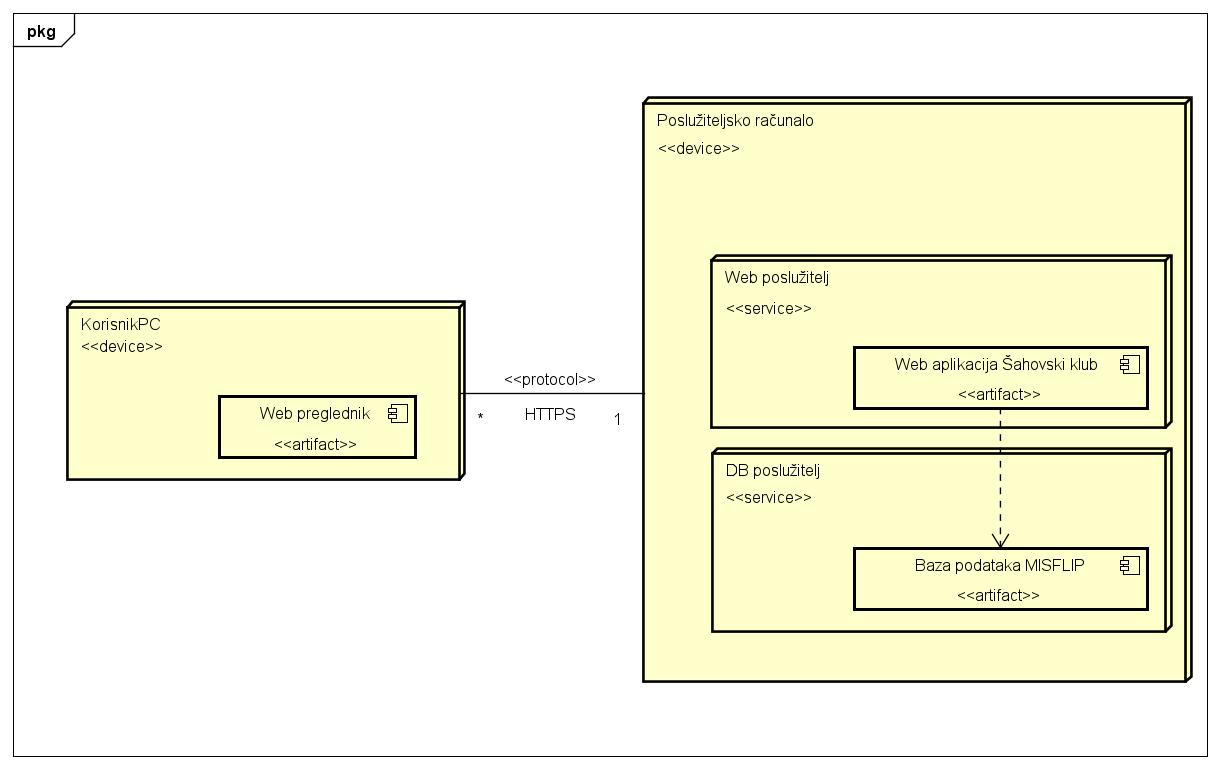
\includegraphics[scale=0.40]{dijagrami/Dijagramrazmjestaja.jpg} %veličina slike u odnosu na originalnu datoteku i pozicija slike
				\caption{Dijagram razmještaja}
				
			\end{figure}
			
			\eject
		
		\section{Upute za puštanje u pogon}
		
			\noindent Za početak potrebno je otići na stranicu \url{https://www.heroku.com/}, registrirati se i prijaviti se s vlastitim korisničkim podacima koji su kreirani putem registracije. 
			
			\noindent U sljedećem koraku treba otvoriti Command Prompt i pozicionirati se u mapu IzvorniKod unutar projekta.
			
			\noindent Potom se upisuje naredba „heroku create“ pri čijem izvršavanju se dobije ime ime servera, a nakon nje „heroku git:remote -a“, i uz ovu naredbu se navodi ime heroku servera koji je dobiven u prethodnom koraku npr. „young-thicket-48718“.
			
			\noindent Nakon toga u datoteku settings.py u ALLOWED\texttt{\char`_}HOSTS treba staviti ime heroku servera i završiti sa ''.herokuapp.com'' npr. ''young-thicket-48718.herokuapp.com''. 
			
			\noindent Nakon što je to napravljeno u Command Promptu upisuje se naredba „git add .“, a poslije nje „git push heroku master“, te je time aplikacija namještena.
			
			
			\eject 